\subsubsection{Iluminação de emergência e sinalização de obstáculos}

	[ ESCREVER UMA INTRODUÇÃO AQUI ]

	\paragraph{Locais de instalação}
	
	Os locais específicos onde se fazem necessária a instalação de sinalização de emergência são:
	
	\begin{figure}[H]
		\centering
		\begin{subfigure}[b]{0.3\textwidth}
			\centering
			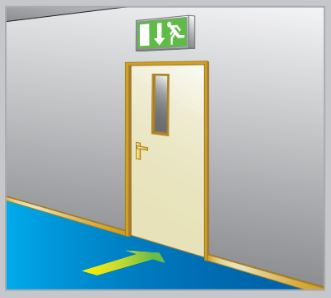
\includegraphics[width=\textwidth]{Figures/3. Lighting/light-safety1.jpg}
			\caption{A cada porta de emergência}
			\label{fig: style 1 image a}
		\end{subfigure}
		\hfill
		\begin{subfigure}[b]{0.3\textwidth}
			\centering
			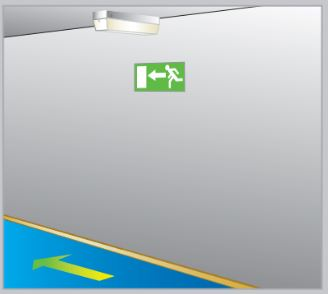
\includegraphics[width=\textwidth]{Figures/3. Lighting/light-safety2.jpg}
			\caption{Todas as sinalizações de saída}
			\label{fig: style 1 image b}
		\end{subfigure}
		\hfill
		\begin{subfigure}[b]{0.3\textwidth}
			\centering
			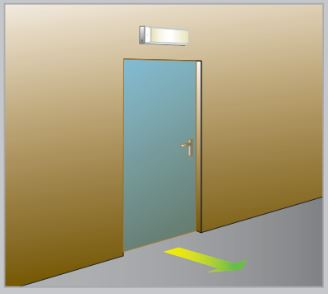
\includegraphics[width=\textwidth]{Figures/3. Lighting/light-safety3.jpg}
			\caption{Nas saídas de emergência}
			\label{fig: style 1 image c}
		\end{subfigure}
	\end{figure}

	\begin{figure}[H]
		\centering
		\begin{subfigure}[b]{0.3\textwidth}
			\centering
			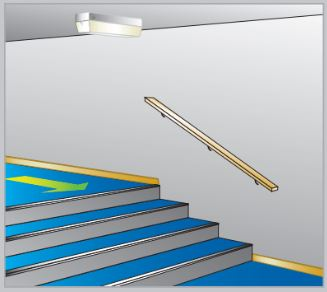
\includegraphics[width=\textwidth]{Figures/3. Lighting/light-safety4.jpg}
			\caption{Próximo escadas}
			\label{fig: style 1 image d}
		\end{subfigure}
		\hfill
		\begin{subfigure}[b]{0.3\textwidth}
			\centering
			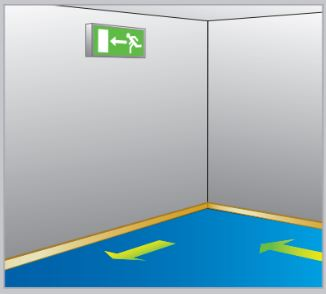
\includegraphics[width=\textwidth]{Figures/3. Lighting/light-safety5.jpg}
			\caption{Nas mudanças de direção}
			\label{fig: style 1 image e}
		\end{subfigure}
		\hfill
		\begin{subfigure}[b]{0.3\textwidth}
			\centering
			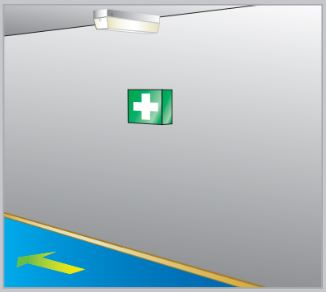
\includegraphics[width=\textwidth]{Figures/3. Lighting/light-safety6.jpg}
			\caption{Nos pontos de primeiro socorros}
			\label{fig: style 1 image f}
		\end{subfigure}
	\end{figure}

	\begin{figure}[H]
		\centering
		\begin{subfigure}[b]{0.3\textwidth}
			\centering
			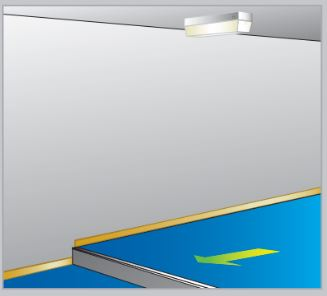
\includegraphics[width=\textwidth]{Figures/3. Lighting/light-safety7.jpg}
			\caption{A cada mudança de nível}
			\label{fig: style 1 image g}
		\end{subfigure}
		\hfill
		\begin{subfigure}[b]{0.3\textwidth}
			\centering
			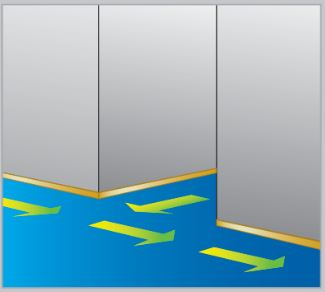
\includegraphics[width=\textwidth]{Figures/3. Lighting/light-safety8.jpg}
			\caption{Nas intersecções dos corredores}
			\label{fig: style 1 image h}
		\end{subfigure}
		\hfill
		\begin{subfigure}[b]{0.3\textwidth}
			\centering
			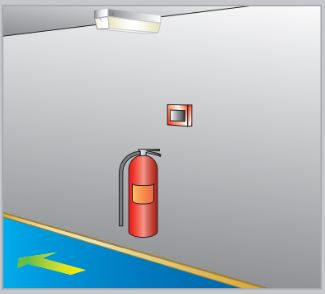
\includegraphics[width=\textwidth]{Figures/3. Lighting/light-safety9.jpg}
			\caption{Próximo a equipamentos de extinção de incêndio}
			\label{fig: style 1 image y}
		\end{subfigure}
		\caption{Localização das luminárias de emergência} - Referência das imagens \cite{eaton2013} 
		\label{fig: safety-luminarires-places}
	\end{figure}
